\newcommand{\content}{
    % добавляем нумерацию
    \AddToShipoutPicture{
        \begin{textblock*}{1cm}(19.5cm,28.6cm) % Ширина блока, координаты (x, y)
                \centering 
                \number\numexpr\thepage+1\relax
        \end{textblock*}
    }

    % добавляем шифр
    \AddToShipoutPicture{
        \begin{textblock*}{10cm}(9cm,28.2cm) % Ширина блока, координаты (x, y)
            \centering
            \chipher
        \end{textblock*}
    }

    % шифр на 1ый лист
    \begin{textblock*}{10cm}(9cm,28.2cm) % Ширина блока, координаты (x, y)
        \centering
        \chipher
    \end{textblock*}

    

\section*{\MakeUppercase{Введение}}
\addcontentsline{toc}{section}{Введение}
    {
        В эпоху цифровых технологий становится очевидным, что искусственный интеллект (ИИ) способен менять способ, которым мы взаимодействуем друг с другом и с окружающим миром. Распознавание эмоций — одна из быстро развивающихся областей, которая позволяет не только анализировать настроение и состояние человека, но и применять эти знания для улучшения пользовательского опыта, коммуникаций и принятия решений.

        Данный проект направлен на создание мобильного приложения, которое сможет определять эмоциональное состояние пользователя на основе анализа изображений лица и текстовых данных. Приложение будет использовать алгоритмы машинного обучения для точного распознавания эмоций, что открывает возможности для его применения в сфере образования, здравоохранения и развлечений.
        Данное мобильное приложение призвано решить следующие задачи:
        \begin{enumerate}
            \item Анализ эмоционального состояния.
            \item Повышение осведомлённости об эмоциях.
            \item Автоматизация процессов анализа настроения.
        \end{enumerate}

        После установки пользователь сможет определять эмоции в реальном времени. Система обрабатывает данные с использованием предварительно обученных моделей глубокого обучения. Для анализа изображений применяется технология компьютерного зрения, которая выделяет ключевые точки лица и классифицирует их в определённые эмоциональные категории, такие как счастье, гнев или удивление.

        История запросов сохраняется в локальной базе данных, что позволяет пользователю отслеживать изменения своего эмоционального состояния и изучать закономерности. Если запрос уникален, приложение проводит новый анализ, а при повторении используется кэш, что значительно ускоряет работу.
    }
    \newpage

\newpage

\section{\MakeUppercase{Постановка задачи}}


\subsection*{Цель работы}
Разработка мобильного приложения, способного автоматически распознавать эмоциональное состояние человека на основе анализа изображений лица с использованием технологий искусственного интеллекта. Приложение призвано интегрировать современные методы машинного обучения для улучшения взаимодействия пользователя с цифровыми сервисами, повышения осведомлённости о собственных эмоциях и их влиянии на повседневную жизнь.

\subsection*{Основные задачи}
Для достижения цели необходимо решить следующие задачи:
\begin{enumerate}
    \item Обучить нейронную модель для анализа выражений лица и классификации эмоций, таких как радость, грусть, удивление и другие.
    \item Создать удобный и интуитивно понятный интерфейс, позволяющий пользователям легко взаимодействовать с приложением.
    \item Провести тестирование модели и интерфейса на реальных данных, оценить точность распознавания эмоций и удобство использования приложения.
\end{enumerate}

\subsection*{Ожидаемые результаты}
В результате выполнения проекта должно быть разработано мобильное приложение, которое:
\begin{itemize}
    \item определяет эмоции пользователя в реальном времени;
    \item обеспечивает интуитивный интерфейс;
    \item демонстрирует визуальный результат анализа.
\end{itemize}

Данное приложение должно быть интуитивно понятным и удобным в использовании, а также демонстрировать основные преимущества интеграции нейронных сетей в мобильные приложения.

\newpage
  
\section{\MakeUppercase{Выбор и описание используемых инструментов}}
{
    \subsection{Модель машинного обучения}
    В данном проекте для распознавания эмоций человека в реальном времени использовалась модель машинного обучения, созданная с помощью Create ML, части экосистемы Core ML от Apple. Create ML предоставляет инструменты для обучения и оптимизации моделей, которые идеально подходят для работы на устройствах Apple.

\subsubsection*{Обоснование выбора модели}
Выбор Create ML обусловлен следующими преимуществами:
\begin{itemize}
    \item \textbf{оптимизация для устройств Apple.} Модели, созданные с помощью Create ML, эффективно работают на iPhone и iPad благодаря оптимизации для процессоров и GPU Apple;
    \item \textbf{простота использования.} Create ML предоставляет удобный и интуитивно понятный интерфейс для обучения моделей, что упрощает разработку;
    \item \textbf{интеграция с Core ML.} Обученные модели легко интегрируются в мобильные приложения с использованием Core ML, ускоряя процесс разработки;
    \item \textbf{работа на устройстве.} Все вычисления происходят локально, что гарантирует защиту конфиденциальности пользователей и минимизирует задержки.
\end{itemize}

\subsubsection*{Принцип работы модели}

Модель обучена на размеченных данных, содержащих изображения с различными выражениями лиц, что позволяет распознавать эмоции, такие как радость, грусть, злость и другие. В реальном времени она принимает видеопоток с камеры устройства, анализирует каждый кадр, определяя ключевые точки на лице, такие как глаза, брови и рот. Эти данные затем сопоставляются с заранее обученными шаблонами эмоциональных выражений. На основе анализа изображения модель классифицирует эмоцию, а также генерирует вероятность, с которой это выражение соответствует конкретной эмоции.

\subsubsection*{Использование модели в проекте}
В рамках проекта модель выполняет следующие функции:
\begin{itemize}
    \item \textbf{распознавание эмоций.} В реальном времени анализирует выражение лица пользователя через камеру и классифицирует его эмоции;
    \item \textbf{поддержка оффлайн-режима.} Предоставляет пользователю мгновенную обратную связь, делая взаимодействие с приложением интуитивным и удобным;
    \item \textbf{обеспечение интерактивности.} Модель способна создавать уникальные и разнообразные рецепты, что делает приложение более полезным для пользователей.
\end{itemize}

Таким образом, использование Create ML в проекте демонстрирует возможности интеграции современных технологий машинного обучения для создания удобных и высокопроизводительных мобильных приложений.
}
\subsection{Инструменты для реализации пользовательского интерфейса}
Для реализации пользовательского интерфейса (UI) веб-приложения были использованы следующие инструменты и технологии:

\subsubsection*{Swift}
Swift — это основной язык программирования для разработки мобильных приложений под платформу iOS. Он был использован для реализации бизнес-логики приложения, включая обработку пользовательских данных и взаимодействие с моделями машинного обучения. Swift позволяет эффективно работать с низкоуровневыми операциями, а также обеспечивает высокую производительность, что важно для работы с камерой устройства в реальном времени.

\subsubsection*{SwiftUI}
SwiftUI — это декларативный фреймворк от Apple, который используется для создания пользовательских интерфейсов. Он позволил создать интуитивно понятный и отзывчивый интерфейс для мобильного приложения. Благодаря декларативному синтаксису SwiftUI упростил процесс разработки и поддержания интерфейса, а также значительно сократил объем кода. В SwiftUI использовались компоненты для отображения изображения с камеры, вывода распознанной эмоции и отображения уведомлений для пользователя.

\subsubsection*{Особенности реализации UI}
В проекте UI был организован следующим образом:
\begin{itemize}
    \item главная страница приложения содержит кнопку для начала использования камеры;
    \item интерфейс адаптируется под различные устройства, обеспечивая корректное отображение на экранах с разными разрешениями и размерами;
    \item все страницы имеют адаптивный дизайн, обеспечивающий корректное отображение на разных устройствах.
\end{itemize}

Использование Swift и SwiftUI для интерфейса позволило создать приложение с высокой производительностью и удобным пользовательским интерфейсом, которое работает эффективно даже на устройствах с ограниченными ресурсами.

\newpage

\section{\MakeUppercase{Разработка приложения}}
В данном разделе описаны этапы разработки приложения для анализа эмоций пользователя.

\subsection{Обучение и тестирование модели машинного обучения}
{
    В рамках данного проекта настройка модели машинного обучения была выполнена с использованием Create ML, инструмента от Apple, который предоставляет простой и удобный интерфейс для создания моделей. Этот подход позволил исключить необходимость ручного написания кода для обучения модели и сосредоточиться на её интеграции с приложением.

\subsubsection*{Настройка модели}
Для решения задачи распознавания эмоций были выполнены следующие этапы настройки:
\begin{itemize}
    \item \textbf{подготовка данных.} Обучающая выборка состояла из изображений лиц, размеченных по категориям эмоций (радость, грусть, злость и т. д.). Данные предварительно обработаны для обеспечения их совместимости с инструментом Create ML;
    \item \textbf{создание модели.} Модель была обучена на наборе размеченных данных с использованием Create ML. Это автоматизировало выбор гиперпараметров и настройку модели;
    \item \textbf{экспорт модели.} Созданная модель экспортирована в формате Core ML для последующей интеграции в приложение.
\end{itemize}

\subsubsection*{Тестирование модели}
После настройки модели проведено тестирование её работы:
\begin{itemize}
    \item было введено множество тестовых запросов с различными эмоциями для проверки точности и релевантности определения эмоций;
    \item анализировалось, соответствует ли формат ответа требованиям приложения;
    \item проверялась способность модели корректно работать с нестандартными выражениями лица или плохим освещением.
\end{itemize}

\subsubsection*{Результаты тестирования}
Модель успешно прошла все этапы тестирования:
\begin{itemize}
    \item ответы модели оказались релевантными, понятными и визуально структурированными;
    \item модель обрабатывает данные в реальном времени без заметных задержек, что критично для пользовательского опыта;
    \item модель продемонстрировала устойчивую работу даже в условиях сложного освещения или частичной видимости лица.
\end{itemize}

}
\newpage

\subsection{Разработка клиентской части приложения}
{
    Клиентская часть приложения разработана с использованием Swift и SwiftUI для создания современного, удобного и интуитивно понятного интерфейса, который позволяет пользователям взаимодействовать с системой распознавания эмоций в реальном времени.

    \subsubsection*{Структура клиентской части}
    
    Клиентская часть приложения реализована в виде экранов, которые написаны с помощью SwiftUI для динамического формирования контента. Основные компоненты интерфейса включают:
    
    \begin{itemize}
        \item \textbf{Форма ввода данных с камеры:} На главном экране отображается изображение с камеры устройства в режиме реального времени. Это позволяет пользователю наблюдать за процессом распознавания эмоций. Камера активируется при запуске приложения, а результат обработки отображается сразу на экране;
        \item \textbf{результаты анализа эмоций:} В верхней части экрана отображаются текущие эмоции пользователя в формате текстовых подсказок и графических элементов. Данные обновляются в реальном времени благодаря встроенной обработке с использованием Core ML;
        \item \textbf{интерактивные элементы:} Кнопки управления, такие как старт и остановка анализа, стилизованы в соответствии с общей концепцией дизайна.
    \end{itemize}
    
    \subsubsection*{Интерактивность и визуальная часть}
    
    Визуальная часть клиентской части приложения включает стилизацию экранов с помощью SwiftUI. Все элементы интерфейса, такие как формы, кнопки были стилизованы для удобства пользователя и обеспечения привлекательного и современного вида. Основные задачи, которые решались на уровне визуализации:
    
    \begin{itemize}
        \item \textbf{SwiftUI для пользовательского интерфейса:} Использование SwiftUI позволило создать декларативный интерфейс с простыми и читаемыми компонентами. Все элементы, такие как кнопки и метки, были оформлены с акцентом на интуитивность и удобство;
        \item \textbf{адаптивный дизайн:} Приложение корректно отображается на устройствах с разными размерами экрана, включая iPhone и iPad. SwiftUI автоматически адаптирует компоненты интерфейса под доступное пространство;
        \item \textbf{анимация и переходы:} Для улучшения восприятия приложения добавлены плавные анимации при переключении экранов или изменении состояния интерфейса.
    \end{itemize}
    
    Для обеспечения интерактивности были использованы базовые возможности SwiftUI. Например, динамическое обновление экрана при определении смены эмоций.
    
    \subsubsection*{Экраны и их функциональность}
    
    Приложение состоит из нескольких ключевых экранов:
    
    \begin{itemize}
        \item \textbf{главный экран:} Содержит кнопку для перехода в режим камеры (см. рис. 3.1);
        \item \textbf{экран камеры:} Экран на котором в реальном времени показывается картинка с камеры и отображается текущая распознаная эмоция (см. рис. 3.2);
    \end{itemize}
    \begin{figure}[H]
        \centering
        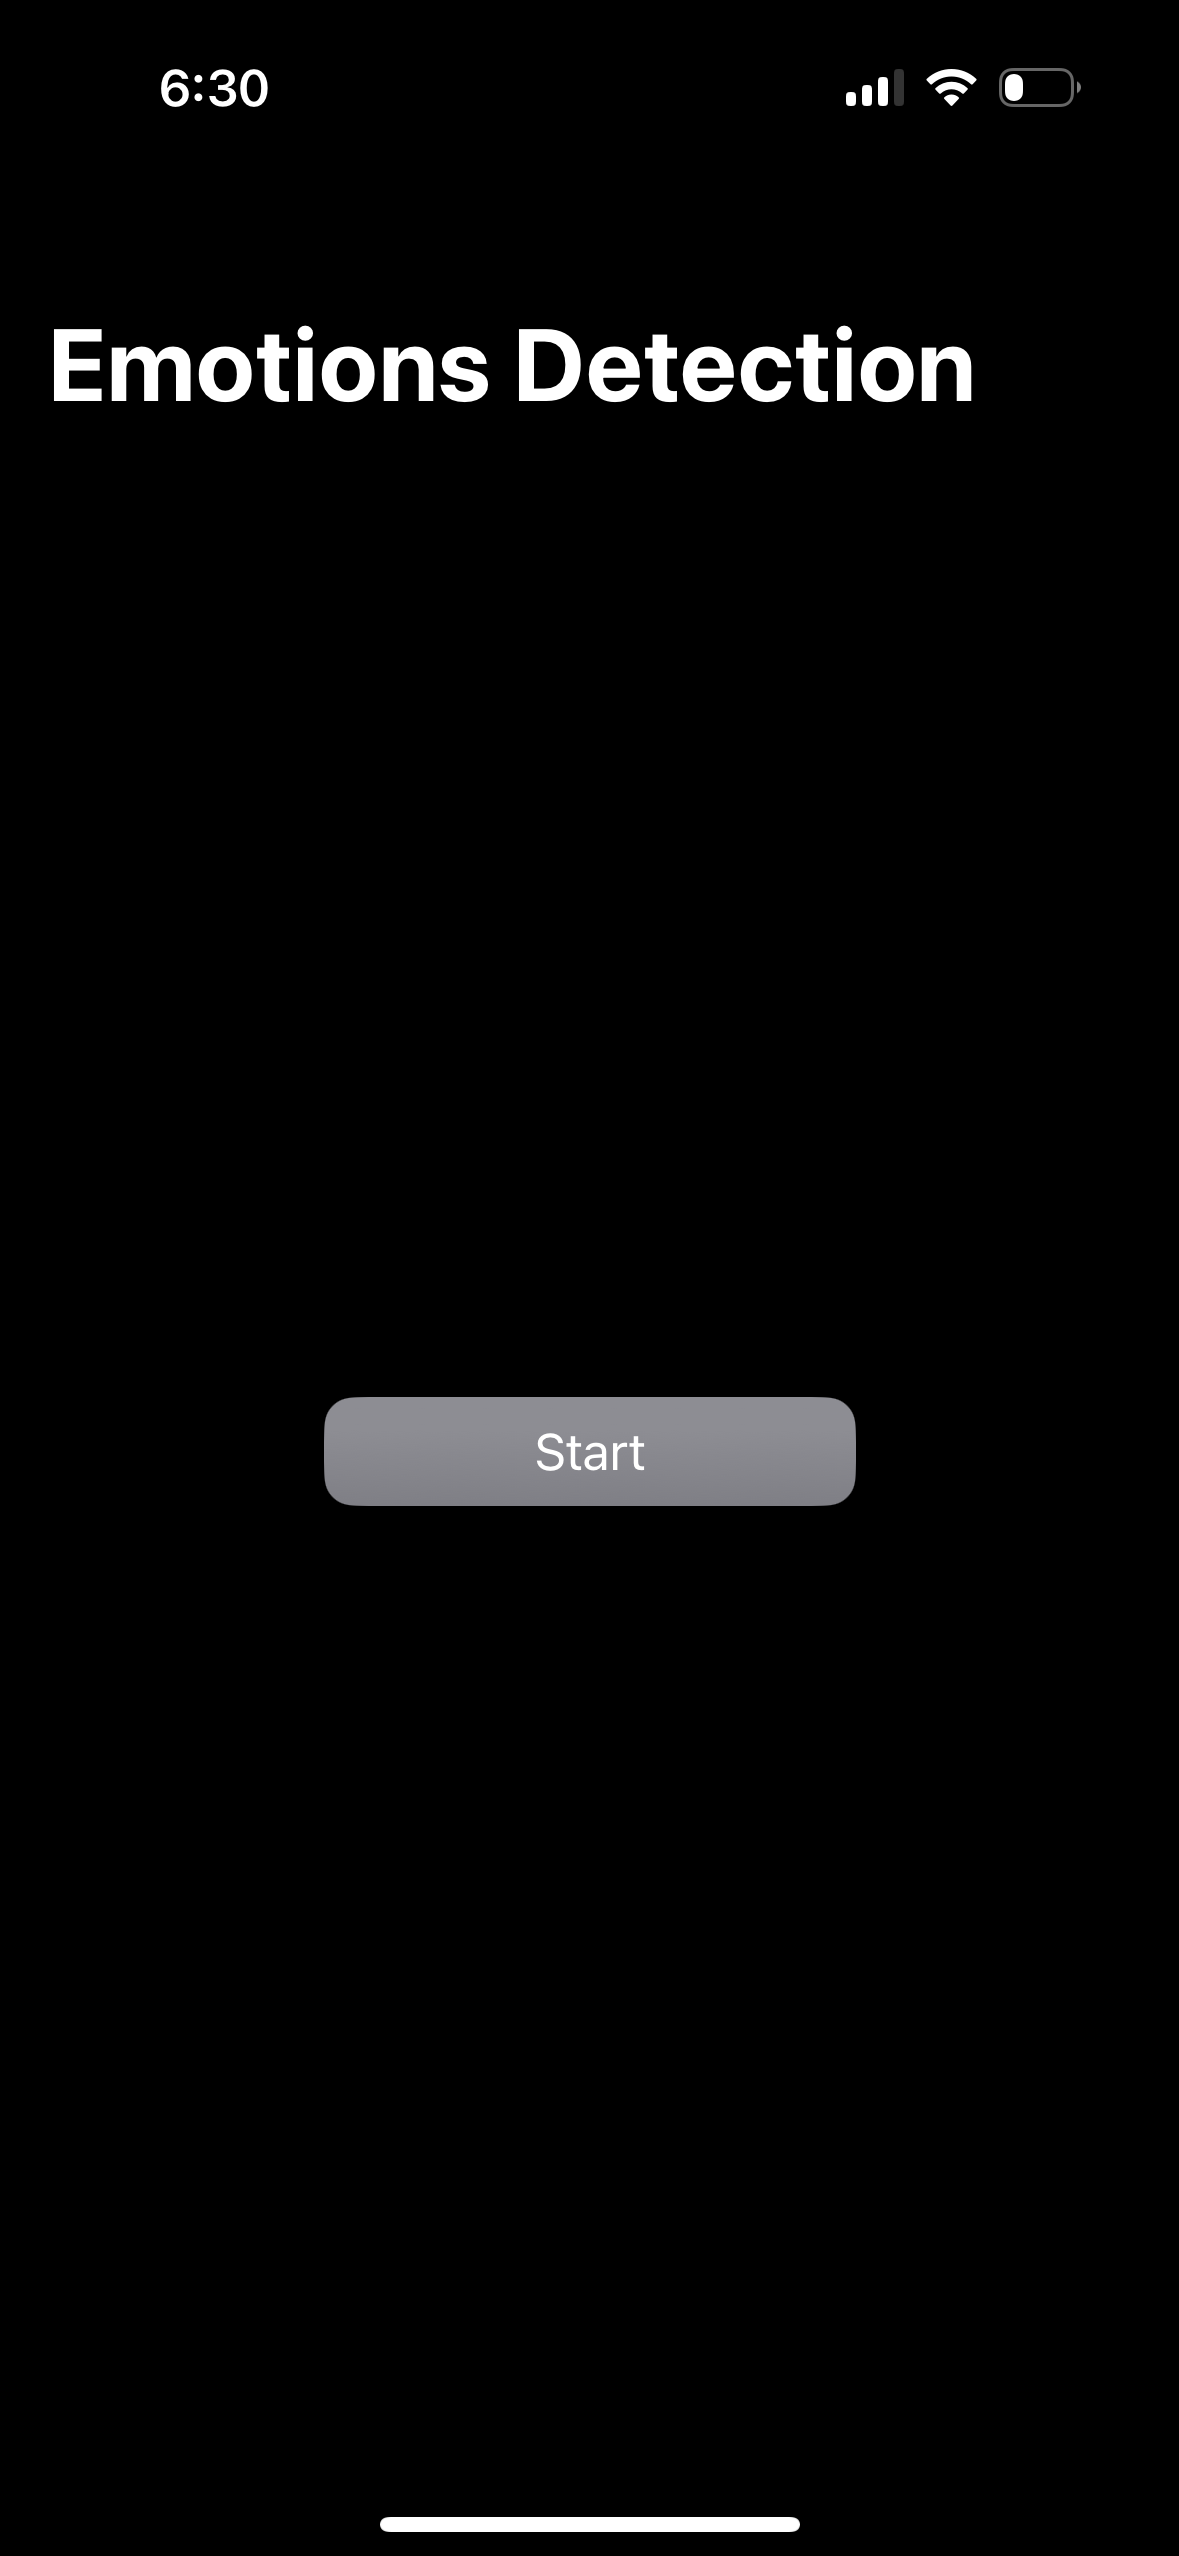
\includegraphics[width=0.3\textwidth]{assets/registration.png} 
        \caption{Главный экран}
    \end{figure}
    \begin{figure}[H]
        \centering
        \includegraphics[width=0.3\textwidth]{assets/index.png} 
        \caption{Экран с камерой}
    \end{figure}
    
    \subsubsection*{Обработка ошибок и сообщений}
    
    Для повышения удобства использования были внедрены сообщения об ошибках и успешных действиях. Например, если произошла ошибка в процессе распознавания эмоций, пользователю отображается уведомление. Такие сообщения помогают быстро идентифицировать проблему и исправить её. Ошибки, такие как неподдерживаемый формат файла или проблемы с анализом данных, наглядно сообщаются, чтобы пользователь мог предпринять необходимые шаги для их устранения.
    
    \subsubsection*{Технологии и инструменты}
    
    Клиентская часть приложения была разработана с использованием SwiftUI, современного фреймворка от Apple, который обеспечивает декларативный подход к созданию пользовательских интерфейсов. SwiftUI позволил создать гибкие и адаптивные экраны, которые легко масштабируются под разные размеры устройств и обеспечивают высокую производительность приложения.
    
    Кроме того, SwiftUI обеспечил простую интеграцию с другими инструментами Apple, такими как Core ML для обработки данных машинного обучения и Vision для анализа изображений, что позволило реализовать взаимодействие между клиентской частью и функциональностью модели.
    
}

\newpage

\section{\MakeUppercase{Тестирование приложения}}

Тестирование приложения является важным этапом разработки, так как оно позволяет проверить корректность работы всех компонентов, выявить возможные ошибки и улучшить пользовательский опыт. В процессе тестирования проверялись различные аспекты работы приложения, включая функциональность, производительность и безопасность.

\subsection{Виды тестирования}

В процессе разработки были применены следующие типы тестирования:

\begin{itemize}
    \item \textbf{юнит-тестирование:} Проверялась корректность отдельных функций и методов, включая обработку данных и взаимодействие с моделями машинного обучения. Юнит-тесты помогли выявить логические ошибки и предотвратить их влияние на другие компоненты приложения;
    \item \textbf{интеграционное тестирование:} Осуществлялась проверка взаимодействия различных частей приложения, таких как передача данных между клиентской частью, серверной логикой и моделью анализа эмоций. Особое внимание уделялось сценариям отображения результатов анализа;
    \item \textbf{тестирование пользовательского интерфейса:} Были проведены проверки удобства и доступности интерфейса с участием реальных пользователей. Тестировались основные пользовательские сценарии, включая загрузку изображения, запуск анализа эмоций и просмотр результатов;
    \item \textbf{нагрузочное тестирование:} Оценивалась производительность приложения при одновременной обработке большого количества запросов, чтобы убедиться, что приложение работает стабильно даже при высокой нагрузке;
    \item \textbf{безопасностное тестирование:} Проводилась проверка на уязвимости, включая защиту пользовательских данных от возможных атак. Проверялись механизмы аутентификации и шифрования данных, чтобы обеспечить высокий уровень безопасности.
\end{itemize}

\subsection{Инструменты и методы тестирования}

Для тестирования были использованы следующие инструменты:

\begin{itemize}
    \item \textbf{XCTest:} Для юнит-тестирования и интеграционного тестирования использовалась встроенная система XCTest, предназначенная для Swift. Этот фреймворк позволяет создавать тесты для моделей, представлений и функций, обеспечивая проверку работы всех компонентов приложения в изолированном окружении;
    \item \textbf{SwiftUI Previews:} Для тестирования пользовательского интерфейса использовалась возможность предварительного просмотра в SwiftUI. Это позволяет проверить внешний вид и взаимодействие элементов интерфейса на разных устройствах и разрешениях экрана в реальном времени.
\end{itemize}

\subsection{Результаты тестирования}

\subsubsection*{Юнит-тестирование}
Все юнит-тесты, проверяющие логику работы с базой данных, бизнес-логику и взаимодействие с нейронной сетью, прошли успешно. Все функции, такие как сортировка ингредиентов, проверка существования записей в базе данных и создание новых запросов, работают корректно.

\subsubsection*{Интеграционное тестирование}
Интеграционные тесты показали, что все компоненты приложения работают правильно в совокупности. Были протестированы сценарии с дублирующимися запросами и корректной обработкой запросов, которые уже были сохранены в базе данных.

\subsubsection*{Тестирование пользовательского интерфейса}
Тестирование интерфейса показало, что экраны приложения интуитивно понятны и удобны для пользователей. Все формы правильно обрабатываются, а результаты запросов корректно отображаются. Были выявлены небольшие улучшения, такие как добавление подсказок и улучшение стилизации для мобильных устройств.

\subsubsection*{Нагрузочное тестирование}
Нагрузочное тестирование показало, что приложение успешно обрабатывает значительное количество запросов без существенного снижения производительности. Однако при резком увеличении числа одновременно поступающих запросов были выявлены области для оптимизации, такие как обработка данных и взаимодействие с хранилищем. В результате были внесены улучшения в алгоритмы работы с данными и увеличена эффективность операций, что значительно повысило быстродействие системы при высокой нагрузке.

\subsubsection*{Безопасностное тестирование}
Безопасностное тестирование выявило ряд потенциальных уязвимостей, включая недостаточную защиту от атак типа CSRF (межсайтовая подделка запросов). Для устранения данных проблем были применены стандартные механизмы безопасности, доступные в SwiftUI, такие как использование токенов защиты сессий и строгие правила проверки данных, передаваемых между клиентом и сервером. Эти меры повысили надежность приложения, обеспечивая защиту пользовательских данных и предотвращая попытки несанкционированного доступа.

\subsection{Заключение по тестированию}

Тестирование показало, что приложение функционирует стабильно и соответствует требованиям, предъявляемым к нему в рамках курсового проекта. Все компоненты работают корректно, и приложение безопасно для использования. На основе результатов тестирования были внесены улучшения в работу с базой данных, а также оптимизированы части кода для повышения производительности.

\newpage

\section*{\MakeUppercase{Заключение}}
\addcontentsline{toc}{section}{Заключение}
{
    В рамках работы над курсовым проектом было разработано приложение для распознавания эмоций в реальном времени с использованием нейронных сетей. Приложение анализирует видеопоток с камеры устройства и классифицирует выражения лица на основе предобученной модели. Система в реальном времени отображает результаты анализа, предоставляя пользователю актуальную информацию о распознанных эмоциях.

    Для реализации проекта использовались технологии Swift и SwiftUI, обеспечивающие создание современного, интуитивно понятного интерфейса. Процесс обработки изображений и взаимодействие с нейронной сетью осуществляется локально, что повышает скорость работы и конфиденциальность данных.
    
    В ходе тестирования приложения были проведены проверки корректности работы алгоритмов, производительности при обработке видеопотока и удобства интерфейса. Результаты тестирования позволили выявить и устранить недостатки, а также оптимизировать работу системы для стабильного функционирования в условиях реального времени.
    
    Этот проект позволил углубить знания в области разработки приложений с использованием машинного обучения и работы с нейронными сетями. Итогом стало создание полностью функционирующего приложения, которое может использоваться для образовательных, исследовательских или развлекательных целей.
}
\newpage


\section*{Список использованной литературы}
\addcontentsline{toc}{section}{Список использованной литературы}
    \sloppy
    {
        \begin{enumerate}
           \item Apple Developer Documentation. SwiftUI Overview [Электронный ресурс]. – Режим доступа: https://developer.apple.com/documentation/swiftui. – Дата доступа: 19.11.2024.
        \item Goodfellow, Ian; Bengio, Yoshua; Courville, Aaron. Deep Learning [Электронный ресурс]. – Режим доступа: https://www.deeplearningbook.org/. – Дата доступа: 19.11.2024.
        \item OpenCV Documentation. Real-Time Emotion Recognition [Электронный ресурс]. – Режим доступа: https://opencv.org/. – Дата доступа: 19.11.2024.  
        \item Stanford University. CS231n: Convolutional Neural Networks for Visual Recognition [Электронный ресурс]. – Режим доступа: http://cs231n.stanford.edu/. – Дата доступа: 19.11.2024.  

        \end{enumerate}
    }

}